\input{./_path-to-root.ltx}
\documentclass[\PathToRoot/\ProjectName]{subfiles}
\whenstandalone{\externaldocument{\PathToRoot/\ProjectName}}

\begin{document}

\begin{figure}[H]
  \centering
  \caption{Model fit to spending behavior and wealth distribution}
  \whenintegrated{\label{fig:splurge_estimation}} 
  \noindent\begin{minipage}{\textwidth}
    \centering
    \begin{subfigure}[b]{.48\linewidth}
      \centering
      % \includegraphics[width=\linewidth]{\PathToRoot/Code/HA-Models/Target_AggMPCX_LiquWealth/Figures/AggMPC_LotteryWin_comparison}
      \includegraphics[width=\linewidth]{\PathToRoot/images/AggMPC_LotteryWin_comparison}
      \caption{Spending dynamics after lottery win}
      \whenintegrated{\label{fig:aggmpclotterywin}} 
    \end{subfigure}
    %
    \hfill
    \begin{subfigure}[b]{.48\linewidth}
      \centering
      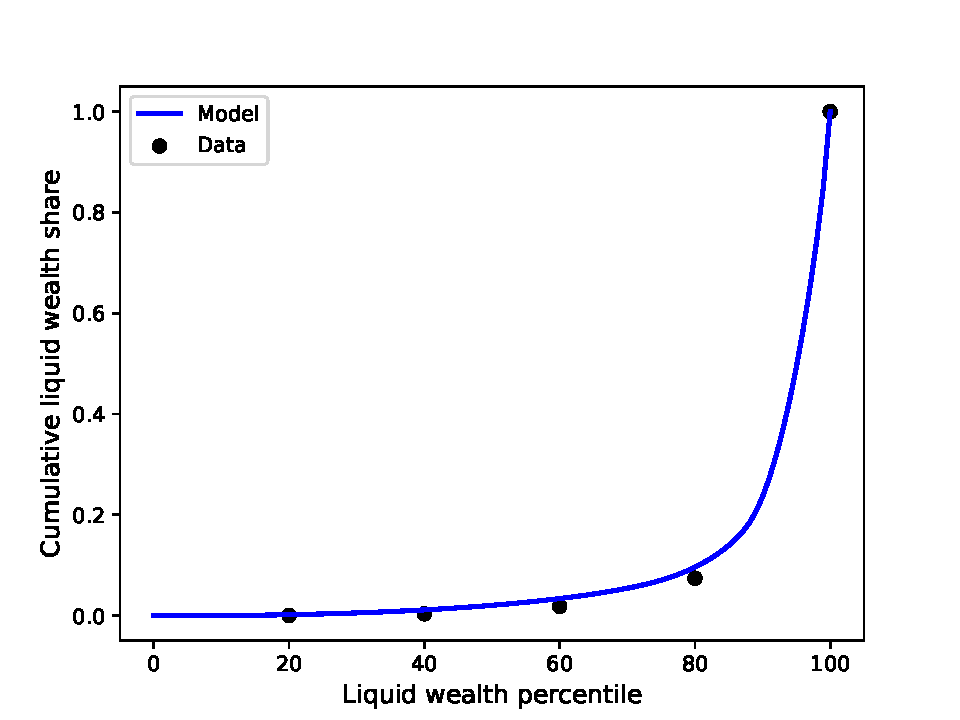
\includegraphics[width=\linewidth]{\PathToRoot/images/LiquWealth_Distribution_comparison}
      \caption{Liquid wealth distribution}
      \whenintegrated{\label{fig:liquwealthdistribution}} 
    \end{subfigure}
  \end{minipage}
\end{figure}
\noindent\parbox{\textwidth}{\footnotesize
  \textbf{Note}: This figure demonstrates the calibration of the splurge factor (Section~\ref{sec:splurge}).
  Panel~(a) shows the model's fit to the dynamic consumption response following lottery wins in Norway,
  as estimated by \cite{fagereng-mpc-2021} using millions of population registry records.
  The splurge factor of $\varsigma = 0.249$ allows the model to match both the high initial MPC
  and the gradual spending over subsequent years.
  Panel~(b) shows the model's fit to the U.S. liquid wealth distribution from the 2004 SCF,
  with 92.6\% of liquid wealth held by the top income quintile.
  See Section~\ref{sec:SCFdata} for the liquid wealth definition following \cite{kaplan2014model}.
}

\vspace{0.5em}  

% Smart bibliography: Only include bibliography if standalone AND has citations  
\smartbib

\end{document}
